\spaltenanfang
Wie immer gibt es noch mehr Meinungen als unsere und eure zum Thema was Informatik ist.
Und da es an der Uni immer gut ist die Meinungen der Professoren zu wissen, haben wir sie mal dazu gefragt.
(Und mit wir meinen wir Grzegorz, der die Interviews damals gemacht hat. Danke Grzegorz!)

\begin{flushleft}\underline{Interview mit Prof. Schnitger} \end{flushleft}

\begin{description}

\item[Fachschaft] 

Was bedeutet für Sie der Begriff Informatik?

\item[Prof. Schnitger]
 
\textit{Wissenschaft der Information.}

\item[Fachschaft]

Was war Ihre Motivation Mathematik zu studieren?

\item[Prof. Schnitger]

\textit{Es ist immer klar worum es geht: Abenteuer im Kopf.}

\item[Fachschaft]

Was fasziniert Sie heutzutage an der Informatik?

\item[Prof. Schnitger]

\textit{Vieles beruht auf der Verarbeitung von Informationen: physikalische Prozesse, Steuerung durch Genom, ...}

\item[Fachschaft]

Welche Tipps können Sie aus Ihrer eigenen Zeit Erstsemestern für das Studium geben?

\item[Prof. Schnitger]

\textit{Arbeiten, arbeiten, ..., und Spaß haben.}

\end{description}
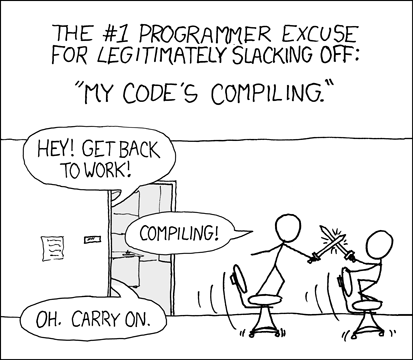
\includegraphics[width=0.95\linewidth]{comics/compiling.png}


\begin{flushleft}\underline{Interview mit Prof. Schmidt-Schauß} \end{flushleft}

\begin{description}

\item[Fachschaft] 

Was bedeutet für Sie der Begriff Informatik?

\item[Prof. Schmidt-Schauß]
 
\textit{Alles was mit  Berechnung, mit Rechnern und Informationsverarbeitung zu tun hat.}

\item[Fachschaft]

Was war Ihre Motivation Mathematik zu studieren?

\item[Prof. Schmidt-Schauß]

\textit{Mathematik war mein Interessengebiet. Mit Computern hatte ich zum ersten mal im vierten Semester zu tun im Numerik Praktikum.}

\item[Fachschaft]

Was fasziniert Sie heutzutage an der Informatik?

\item[Prof. Schmidt-Schauß]

\textit{Informatik bzw. Computer sind relevant in immer mehr Bereichen des Lebens, Technik und Wissenschaft.
Informatik ist eine junge Wissenschaft und es gibt dort noch zahlreiche offene und interessante Probleme zu lösen.}

\item[Fachschaft]

Welche Tipps können Sie aus Ihrer eigenen Zeit Erstsemestern für das Studium geben?

\item[Prof. Schmidt-Schauß]

\textit{Grundlagen der Informatik in jeder Form sind wichtig (nicht beschränkt auf die entsprechende Vorlesung). Später im Berufsleben gibt es so gut wie keine Zeit mehr, die Theorie, die jetzt leicht zu lernen ist, nochmals nachzuholen.}

\end{description}


\begin{flushleft}\underline{Interview mit Prof. Hedrich} \end{flushleft}

\begin{description}

\item[Fachschaft] 

Was bedeutet für Sie der Begriff Informatik?

\item[Prof. Hedrich]
 
\textit{Informatik ist die Wissenschaft der Informationsverarbeitung im Allgemeinen.
Sie ist durch die rasante Entwicklung in der Computertechnik zu einer sehr
bedeutsamen Wissenschaft geworden und weist damit sehr viele unterschiedliche, 
interessante Zweige auf. Von der Robotik bis hin zur Logik und Komplexitätstheorie.}


%\includegraphics[width=\linewidth]{comics/FuturamaComics/Comicsfinal/Studienwahl4voll}

\item[Fachschaft]

Was war Ihre Motivation Elektrotechnik zu studieren?

\item[Prof. Hedrich]

\textit{Während des Studiums konnte ich mein Interesse für die Computer (ich hab
in der Schule mit einem Commodore PET angefangen und mich dann in
die C64 Technik vertieft) mit dem für Elektrotechnik verbinden.
So kam es zu meinem Forschungsinteressen, den rechnergestützten Entwurf von
Schaltungen.}

\item[Fachschaft]

Was fasziniert Sie heutzutage an der Informatik?

\item[Prof. Hedrich]

\textit{Das weite Anwendungsfeld und besonders auch die großen
Gestaltungsmöglichkeiten, da Informatik ja inzwischen fast überall
zu finden ist. Speziell finde ich natürlich die technischen Entwicklungen
spannend z.B. den aktuellen Umstieg von Single-Prozessorsystemen auf
Multi-Cores bis hin zu 800 Prozessoren auf einer Grafikkarte für
jedermann.}

\item[Fachschaft]

Welche Tipps können Sie aus Ihrer eigenen Zeit Erstsemestern für das Studium geben?

\item[Prof. Hedrich]

\textit{Schauen Sie sich die Vorlesungen an. Es kann sowohl fachlich als auch
menschlich interessant sein. Ein guter Studienkommilitone hilft enorm,
sowohl bei der Auswahl der richtigen Veranstaltungen als auch während der
ganzen Lernerei. Und ein bisschen Entspannung bei einer Fete ist am Ende einer Woche
auch nicht verkehrt.}

\end{description}


%\includegraphics[width=\linewidth]{comics/FuturamaComics/Comicsfinal/Studienwahl5voll}

%\begin{flushright} Grzegorz \end{flushright}

\spaltenende
